% Diapositiva 1: ¿Qué es Blender?
\begin{frame}{¿Qué es Blender?}
    \begin{itemize}
        \item Blender es un software de modelado, animación y renderizado 3D de código abierto.
        \item Es utilizado en diversas industrias como animación, efectos visuales, videojuegos y diseño industrial.
        \item Permite modelar objetos 3D con movimiento articulado basado en nodos y operaciones.
        \item Permite modelado poligonal, simulaciones físicas y animación.
    \end{itemize}
    \begin{center}
        \includegraphics[width=0.6\linewidth]{01_Blender/blender.png}
    \end{center}
\end{frame}

% Diapositiva 2: Funcionamiento de Blender
%\begin{frame}{Funcionamiento de Blender}
%    \begin{itemize}
%        \item Basado en un flujo de trabajo no destructivo con modificadores y nodos.
%        \item Permite modelado poligonal, esculpido digital, animación y simulaciones físicas.
%        \item Motor de renderizado Cycles y Eevee para resultados realistas y en tiempo real.
%        \item Compatibilidad con scripting en Python para automatización y personalización.
%    \end{itemize}
%    \begin{center}
%        \includegraphics[width=0.6\linewidth]{01_Blender/blender.png}
%    \end{center}
%\end{frame}

% Diapositiva 3: Aplicaciones de Blender
\begin{frame}{Aplicaciones de Blender}
    \begin{itemize}
        \item \textbf{Animación y cine:} Usado en películas y cortos animados como "Spring" y "Sintel".
        \item \textbf{Videojuegos:} Creación de modelos y animaciones para motores como Unity y Unreal Engine.
        \item \textbf{Arquitectura y diseño:} Visualización de espacios en 3D con realismo.
        \item \textbf{Impresión 3D:} Modelado y exportación de archivos para fabricación.
    \end{itemize}
    \begin{center}
        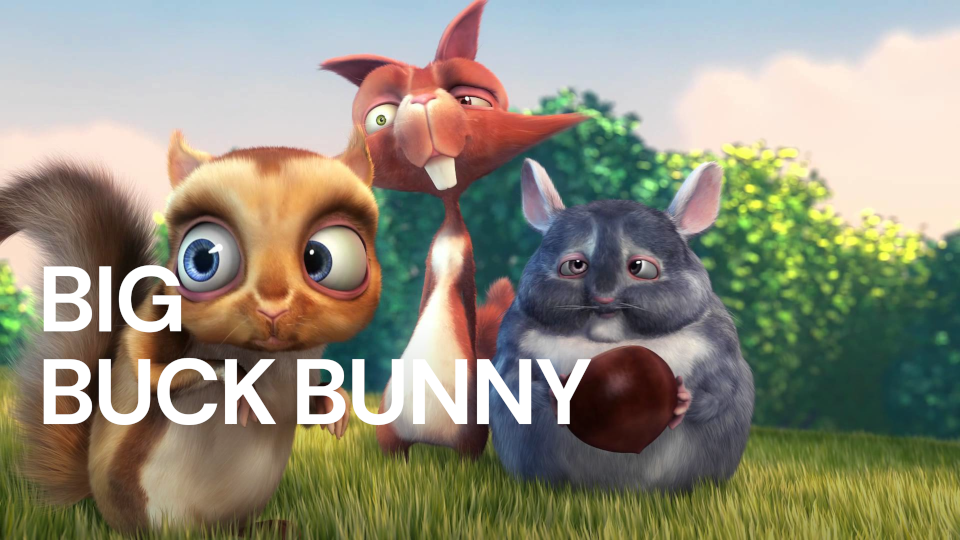
\includegraphics[width=0.6\linewidth]{01_Blender/BigBuckBunny.png}
    \end{center}
\end{frame}
